% ─────────────────────────────────────────────────────────────────────────────
\section{Results and Discussion}
% ─────────────────────────────────────────────────────────────────────────────

One implementation choice shapes all the results because in our simulation, victims are stationary and do not change location after placement. Because the underlying search objective does not change, we set the pheromone evaporation rate to a very low value. Pheromone deposited on a cell effectively persists for the duration of a run, making recently explored territory reliably repulsive. This also explains why the staleness exponent $\beta$ has little measurable effect because cells never genuinely become stale when the state of the world does not change beneath them.

\subsection{Step Length Sweep}

The step length sweep isolates the effect of the planning ring radius on search performance.
Twenty independent random seeds (1--20) are evaluated across eight fixed step lengths
$d \in \{1.25, 2.5, 3.75, 5.0, 6.25, 7.5, 8.75, 10.0\}$\,m.
All other parameters are held at their defaults: $n = 24$ candidate waypoints,
$\alpha = 1.0$, $\beta = 1.0$, and a sensor range of 5\,m.
The adaptive step mechanism is disabled for all fixed-step conditions, ensuring that the
configured ring radius is the one actually used throughout each run.
A ninth condition, the ``Default (adaptive)'' baseline, re-runs the same 20 seeds with
adaptive scaling enabled and a base step of $d = 4$\,m, providing a direct comparison
between fixed and adaptive strategies under otherwise identical settings.

Steps of 2.5 and 5.0\,m achieve the highest convergence rate at 76\,\%, making them jointly
optimal within the evaluated range.
The shortest step ($d = 1.25$\,m) achieves the fastest mean convergence time among runs that
do converge (44.7\,s $\pm$ 14.6\,s SD), but its convergence rate is only 26\,\%,
meaning most runs fail to locate all victims within the time limit.
Steps in the mid-range (3.75--7.5\,m) plateau at 60--76\,\%, with mean convergence times
between 53 and 70\,s and substantial run-to-run variance.
The default adaptive configuration converges on only 45\,\% of seeds with a mean time
of 55.8\,s, underperforming most fixed-step alternatives on both metrics.

\begin{figure}[h]
    \centering
    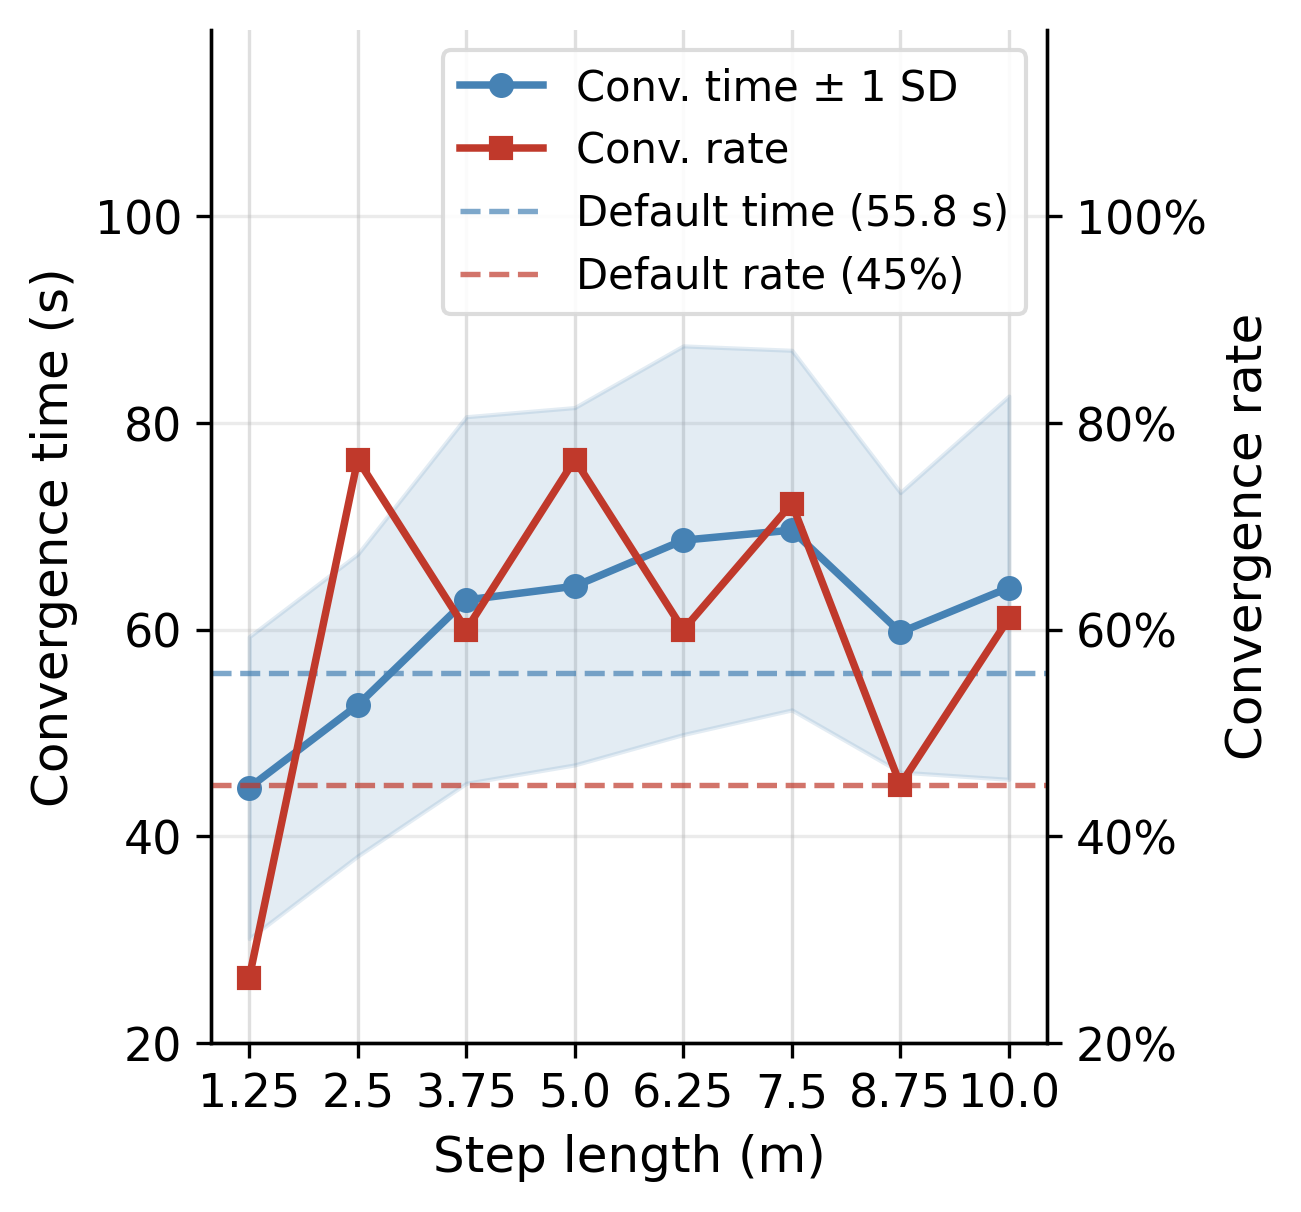
\includegraphics[width=\columnwidth]{img/experiments/step_sweep_plot.png}
    \caption{Convergence rate and mean convergence time ($\pm$1\,SD, converged runs only)
             as a function of fixed step length (20 seeds each).
             Steps of 2.5 and 5.0\,m yield the highest convergence rate (76\,\%).
             The rightmost group is the default configuration with adaptive step scaling
             enabled (base $d = 4$\,m), which achieves only 45\,\% convergence, worse
             than most fixed-step alternatives.}
    \label{fig:step_sweep}
\end{figure}

The shape of the response follows from how step length relates to the sensor range (5m).
Upon arriving at a candidate waypoint, the UAV has already sensed the forward direction
up to 5m ahead throughout its approach.
When new candidates are placed within that radius ($d < 5$m, e.g.\ $d = 1.25$m), the
area directly ahead is already pheromone-marked before any new candidate is ever generated
there.
The scoring function consequently never selects a forward-facing candidate, forcing the
agent into lateral or backward moves at every step.
This produces constant direction reversals rather than coherent coverage, and explains the
low 26\% convergence rate at $d = 1.25$m.
At the opposite extreme ($d \geq 8.75$m), candidates are placed so far from the UAV that
the pheromone values at those positions are entirely unrepresentative of the local coverage
state.
The scoring function no longer encodes a meaningful spatial gradient and directional choice
becomes effectively arbitrary.
The sweet spot at $d \in \{2.5, 5.0\}$m places candidates near the boundary of the sensed
area, where pheromone levels are fresh, locally informative, and varied enough to guide
consistent progress.
The adaptive mechanism underperforms for the same reason as long fixed steps.
Enlarging the ring in response to locally high pheromone density pushes candidates beyond
the sensed neighbourhood, reintroducing the uninformative signal before clusters are fully
confirmed.

\subsection{Full Factorial Sweep}

We evaluate the UAV-SAR model using a full factorial sweep over four key ACO parameters: candidate count, step length, pheromone exponent $\alpha$, and staleness exponent $\beta$. Candidate count is varied over $\{12,18,24,30,36\}$, step length over $\{50,75,100,125,150\}$, $\alpha$ over $\{0.5,1.0,1.5,2.0,2.5\}$, and $\beta$ over $\{1.0,1.5,2.0,2.5,3.0,3.5,4.0\}$. This yields 875 parameter combinations per seed.

We first validate the sweep with 3 seeds before scaling to the full run. The validation batch completed all expected runs (2,625/2,625 rows in \texttt{run\_summary.csv}) with a convergence rate of 95.85\% (2,516 converged, 109 timeouts). After validation, we execute the full 10-seed sweep for a total of 8,750 runs.

The full run also completed all expected parameter-seed combinations (8,750/8,750 rows). Overall convergence is 93.84\% (8,211 converged runs, 539 timeouts). At configuration granularity, 525 out of 875 parameter combinations achieved 100\% convergence across all 10 seeds, indicating a broad robust operating region.

Main effects show that step length is the strongest reliability lever: the shortest step ($d=50$) has the lowest mean convergence rate (0.822), while $d=100$ is highest (0.981). Candidate count is non-monotonic: moderate values ($n \in \{12,18,24\}$) outperform denser rings ($n \in \{30,36\}$). This pattern is consistent with a decentralized exploration-exploitation balance where overly dense local candidate sets can delay global closure.

The visual diagnostics in Figures~\ref{fig:fullfactorial_dashboard}--\ref{fig:fullfactorial_tradeoff} summarize the main structure of the sweep. The dashboard combines the step/candidate reliability map, the $\alpha$--$\beta$ interaction map, the reliability--time trade-off, and the seed-stability profile in a single compact overview. The top-15 bar chart then isolates the fastest fully-converged settings.

\begin{figure*}[ht]
  \centering
  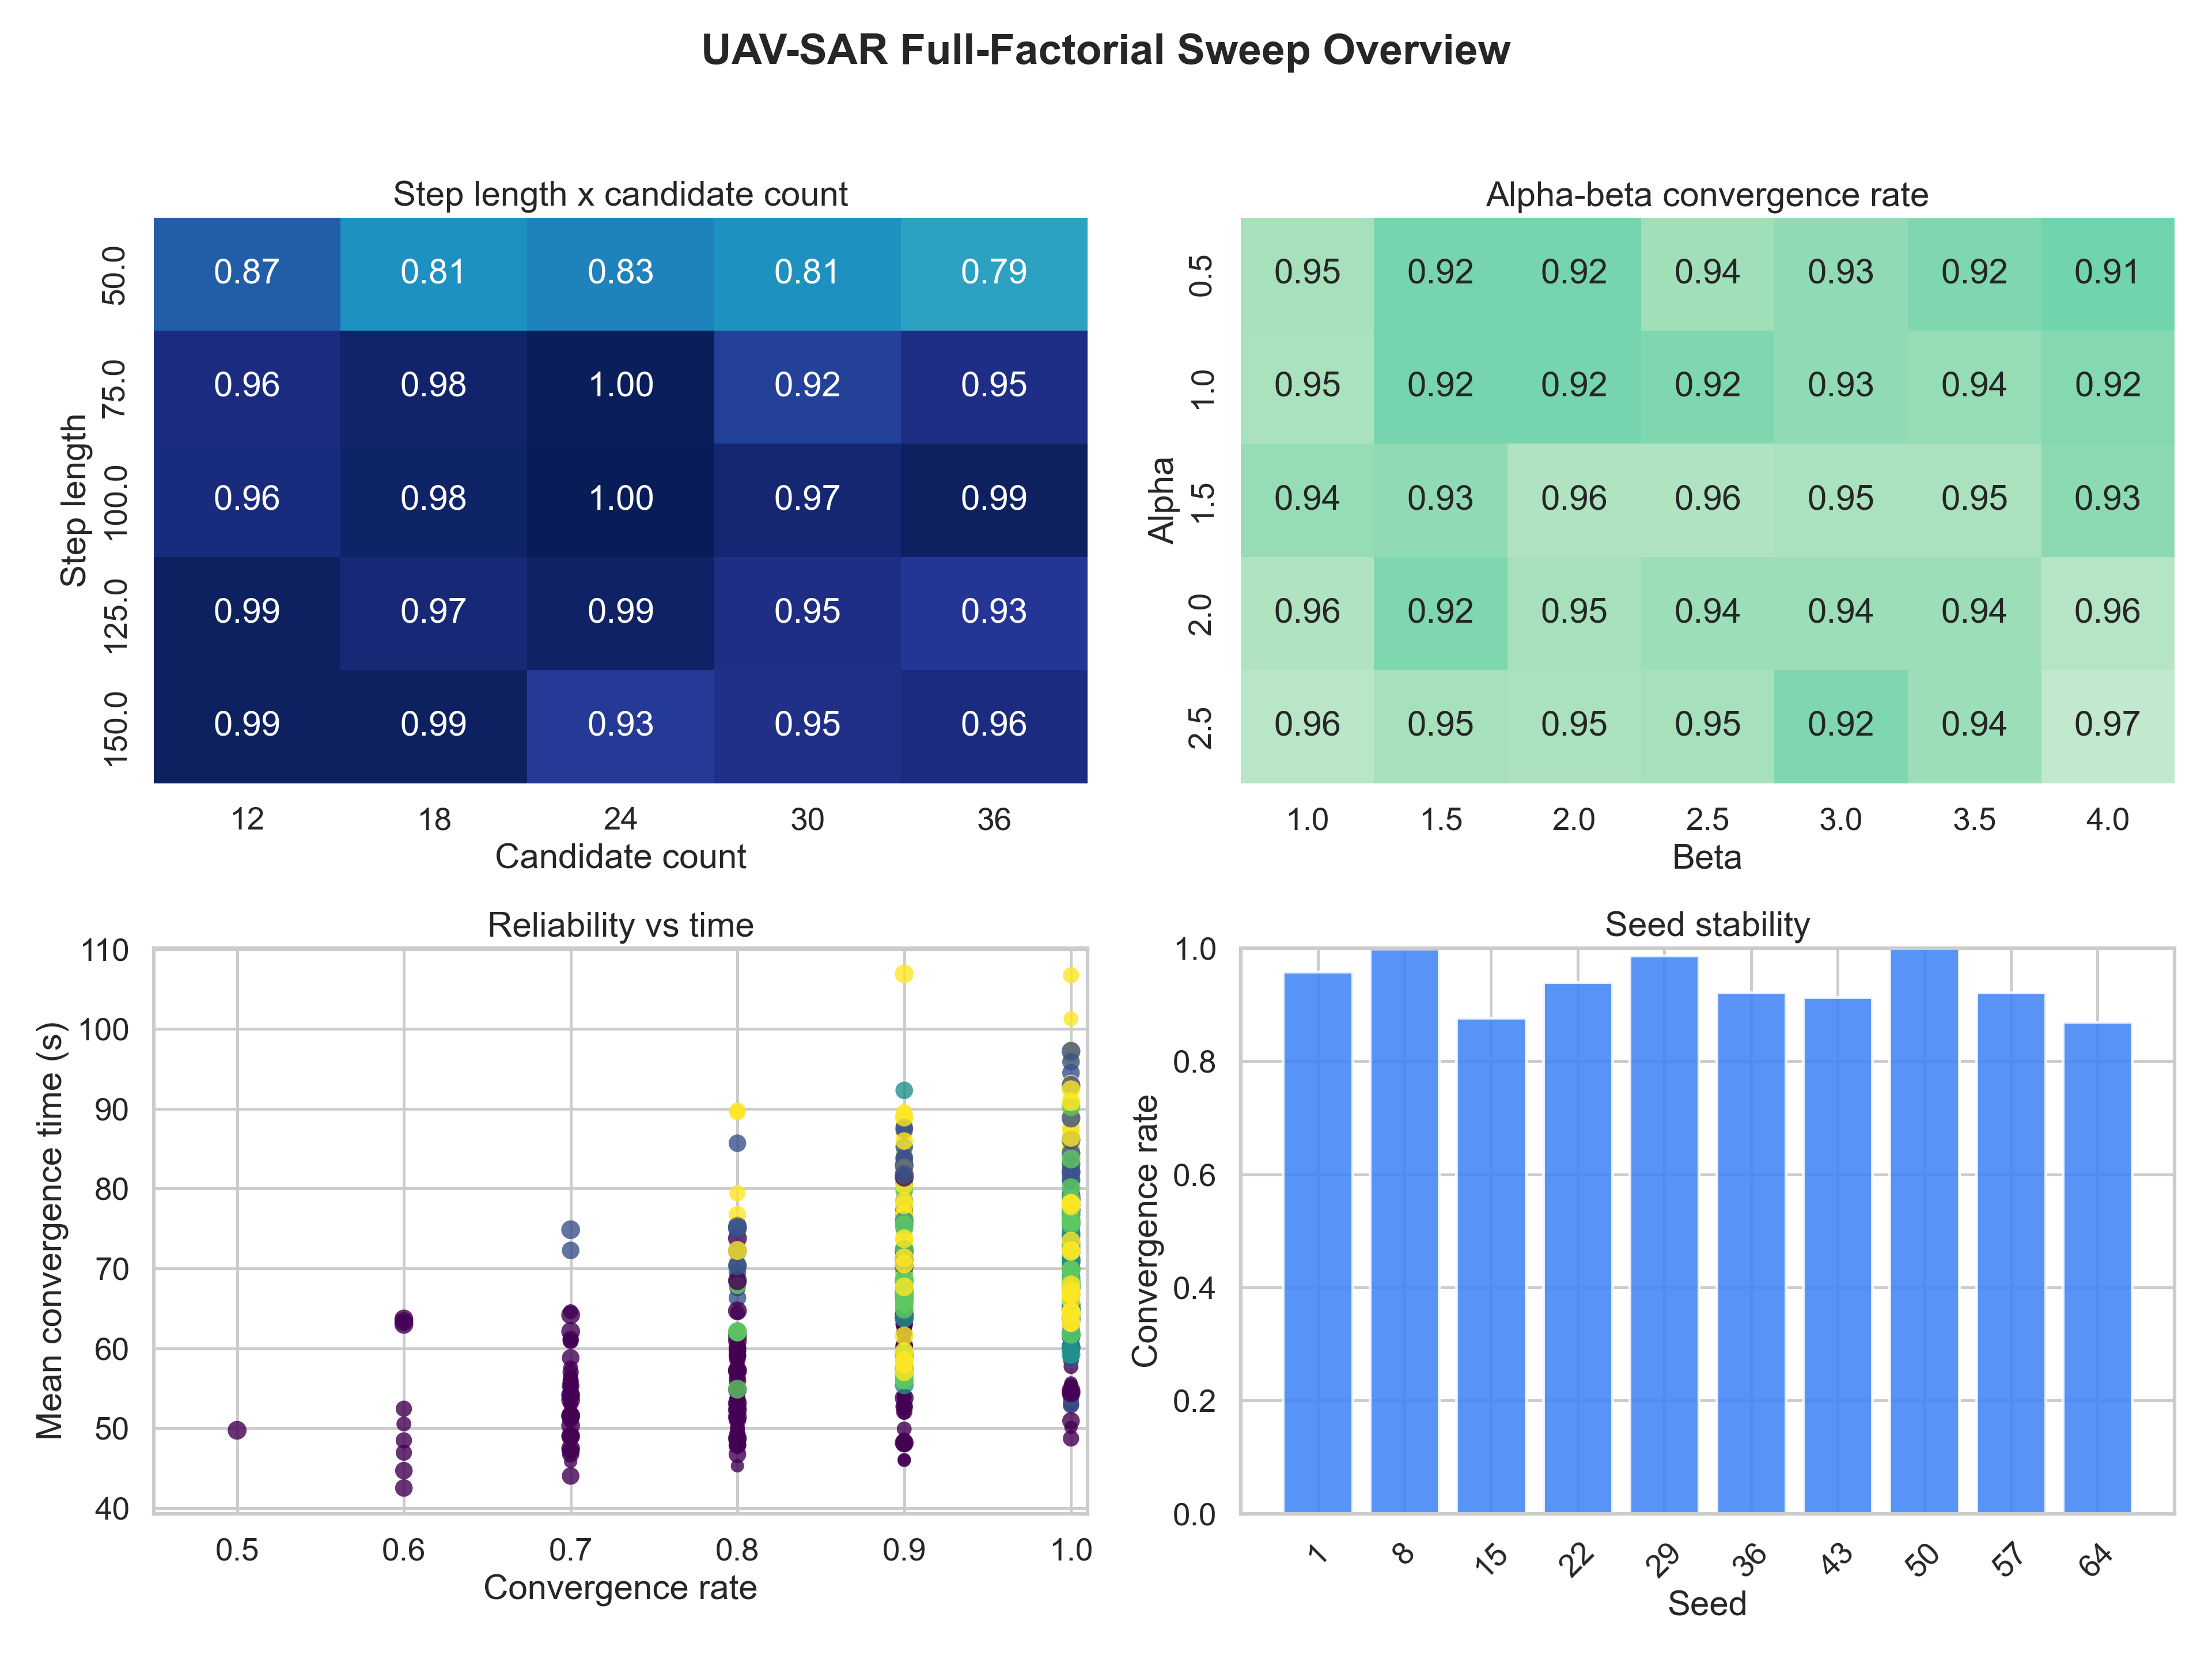
\includegraphics[width=0.92\textwidth]{img/experiments/full_factorial_20260601003651074/full_factorial_dashboard.png}
  \caption{Compact overview of the full-factorial sweep. The four panels summarize the dominant interaction surfaces, the reliability--time trade-off, and the seed-level stability pattern.}
  \label{fig:fullfactorial_dashboard}
\end{figure*}

\begin{figure*}[ht]
    \centering
    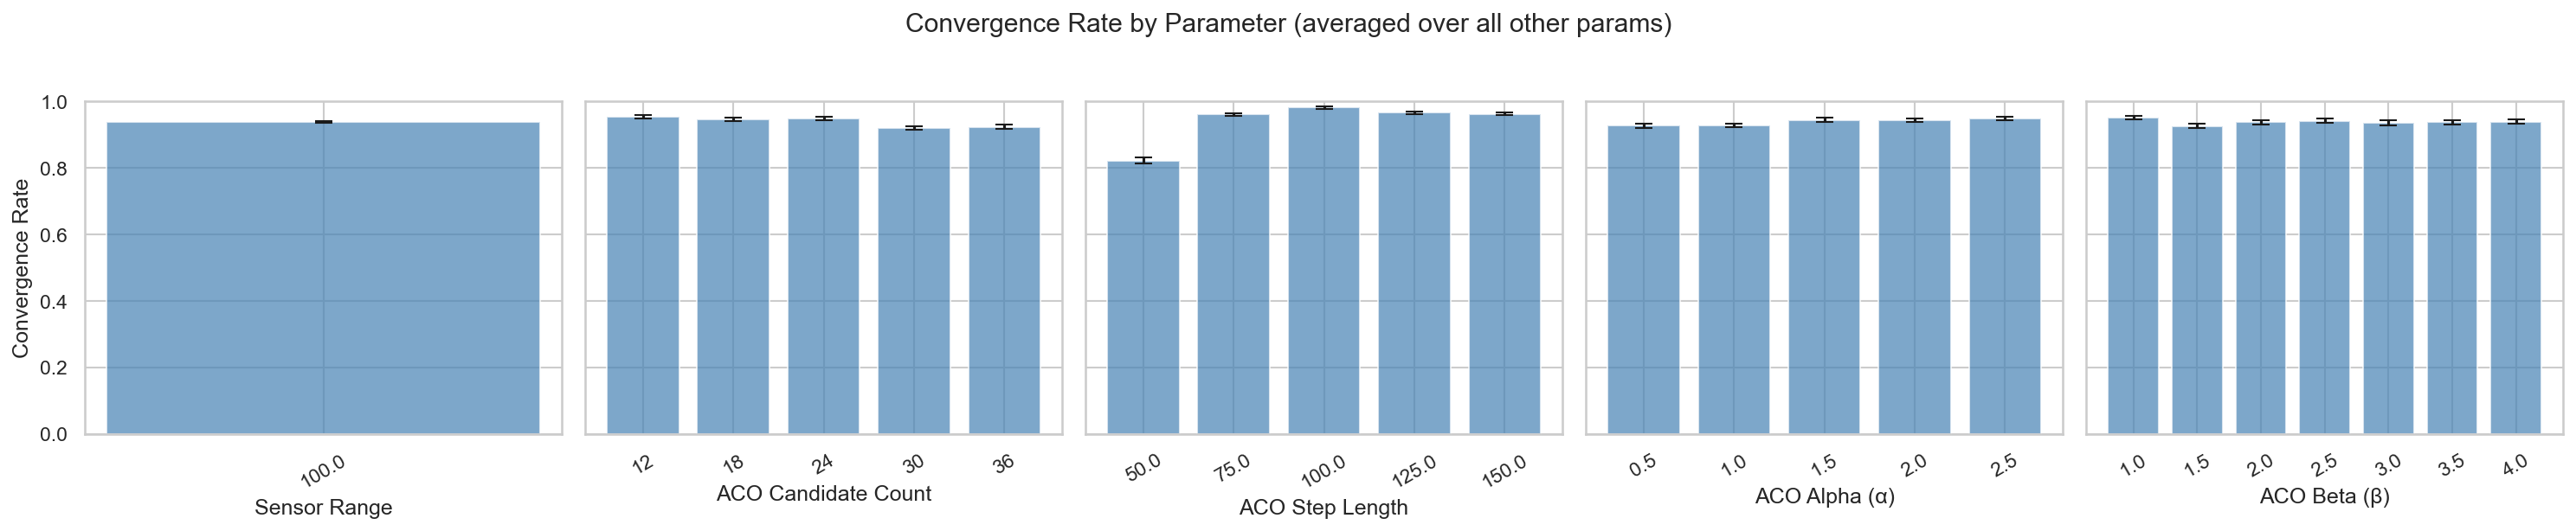
\includegraphics[width=0.49\textwidth]{img/experiments/full_factorial_20260601003651074/marginal_convergence_rate.png}
    \hfill
    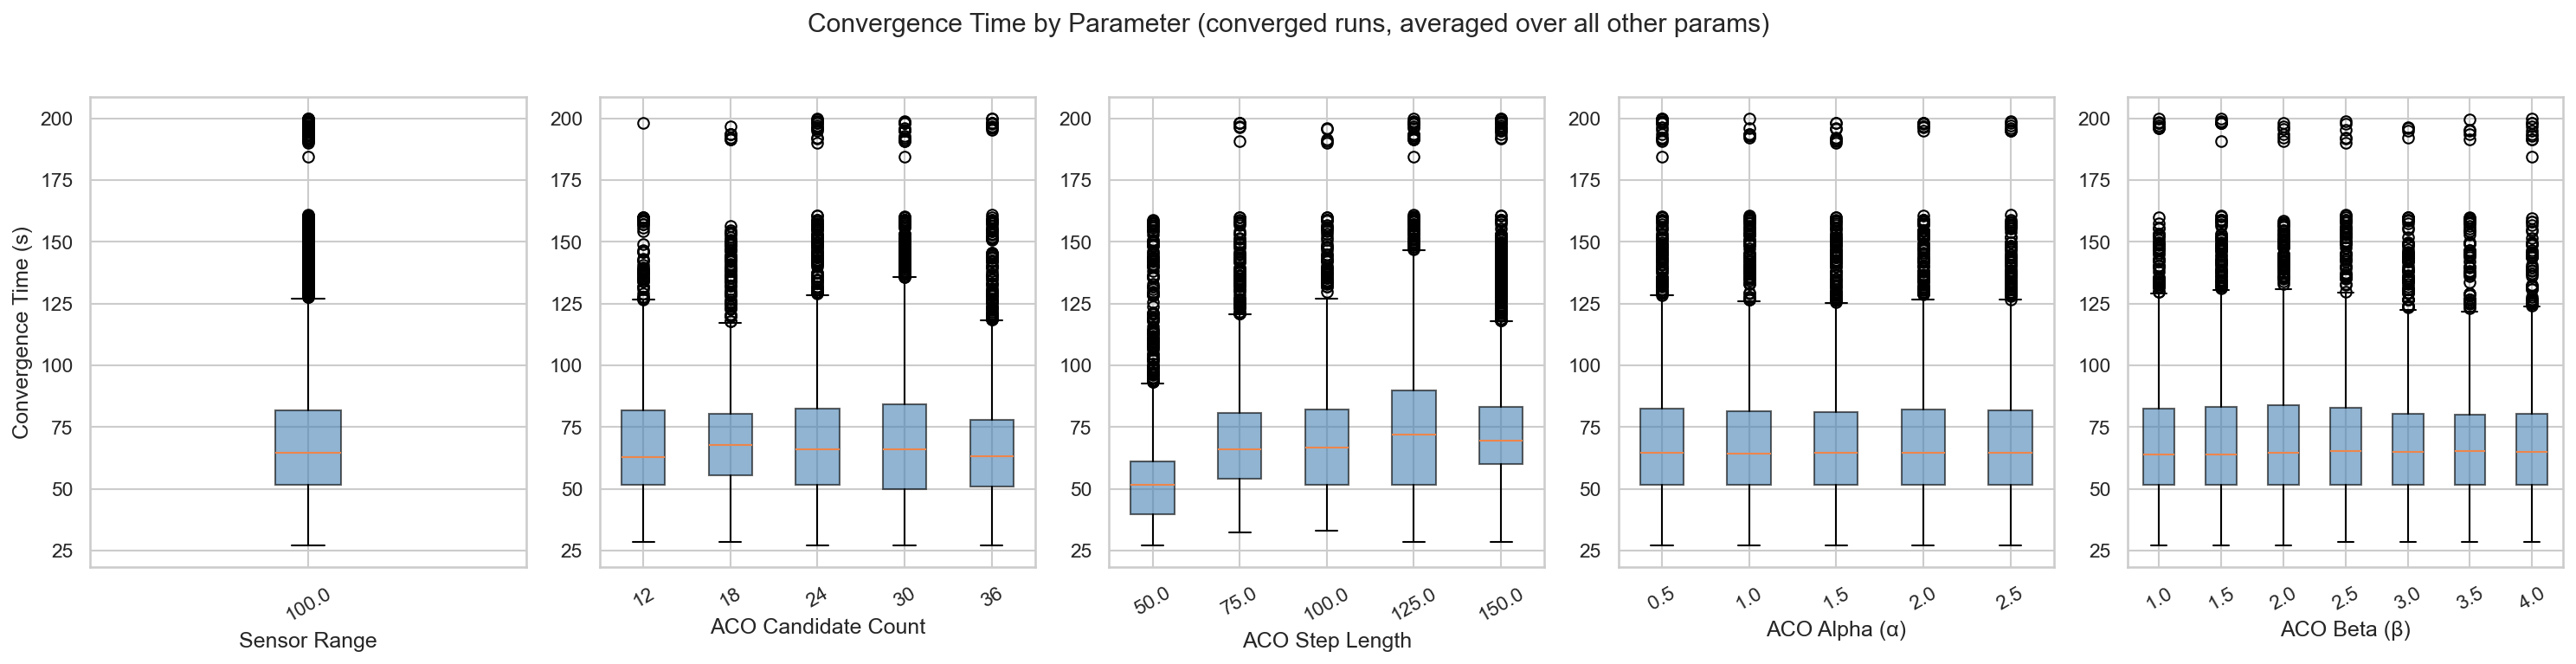
\includegraphics[width=0.49\textwidth]{img/experiments/full_factorial_20260601003651074/marginal_convergence_time.png}
    \caption{Full-factorial marginal effects (8,750 runs). Left: convergence-rate distributions by parameter value. Right: convergence-time distributions for converged runs. Reliability drops sharply at the shortest step length, while intermediate-to-long steps preserve high completion rates.}
    \label{fig:fullfactorial_marginals}
\end{figure*}

\begin{figure*}[ht]
    \centering
    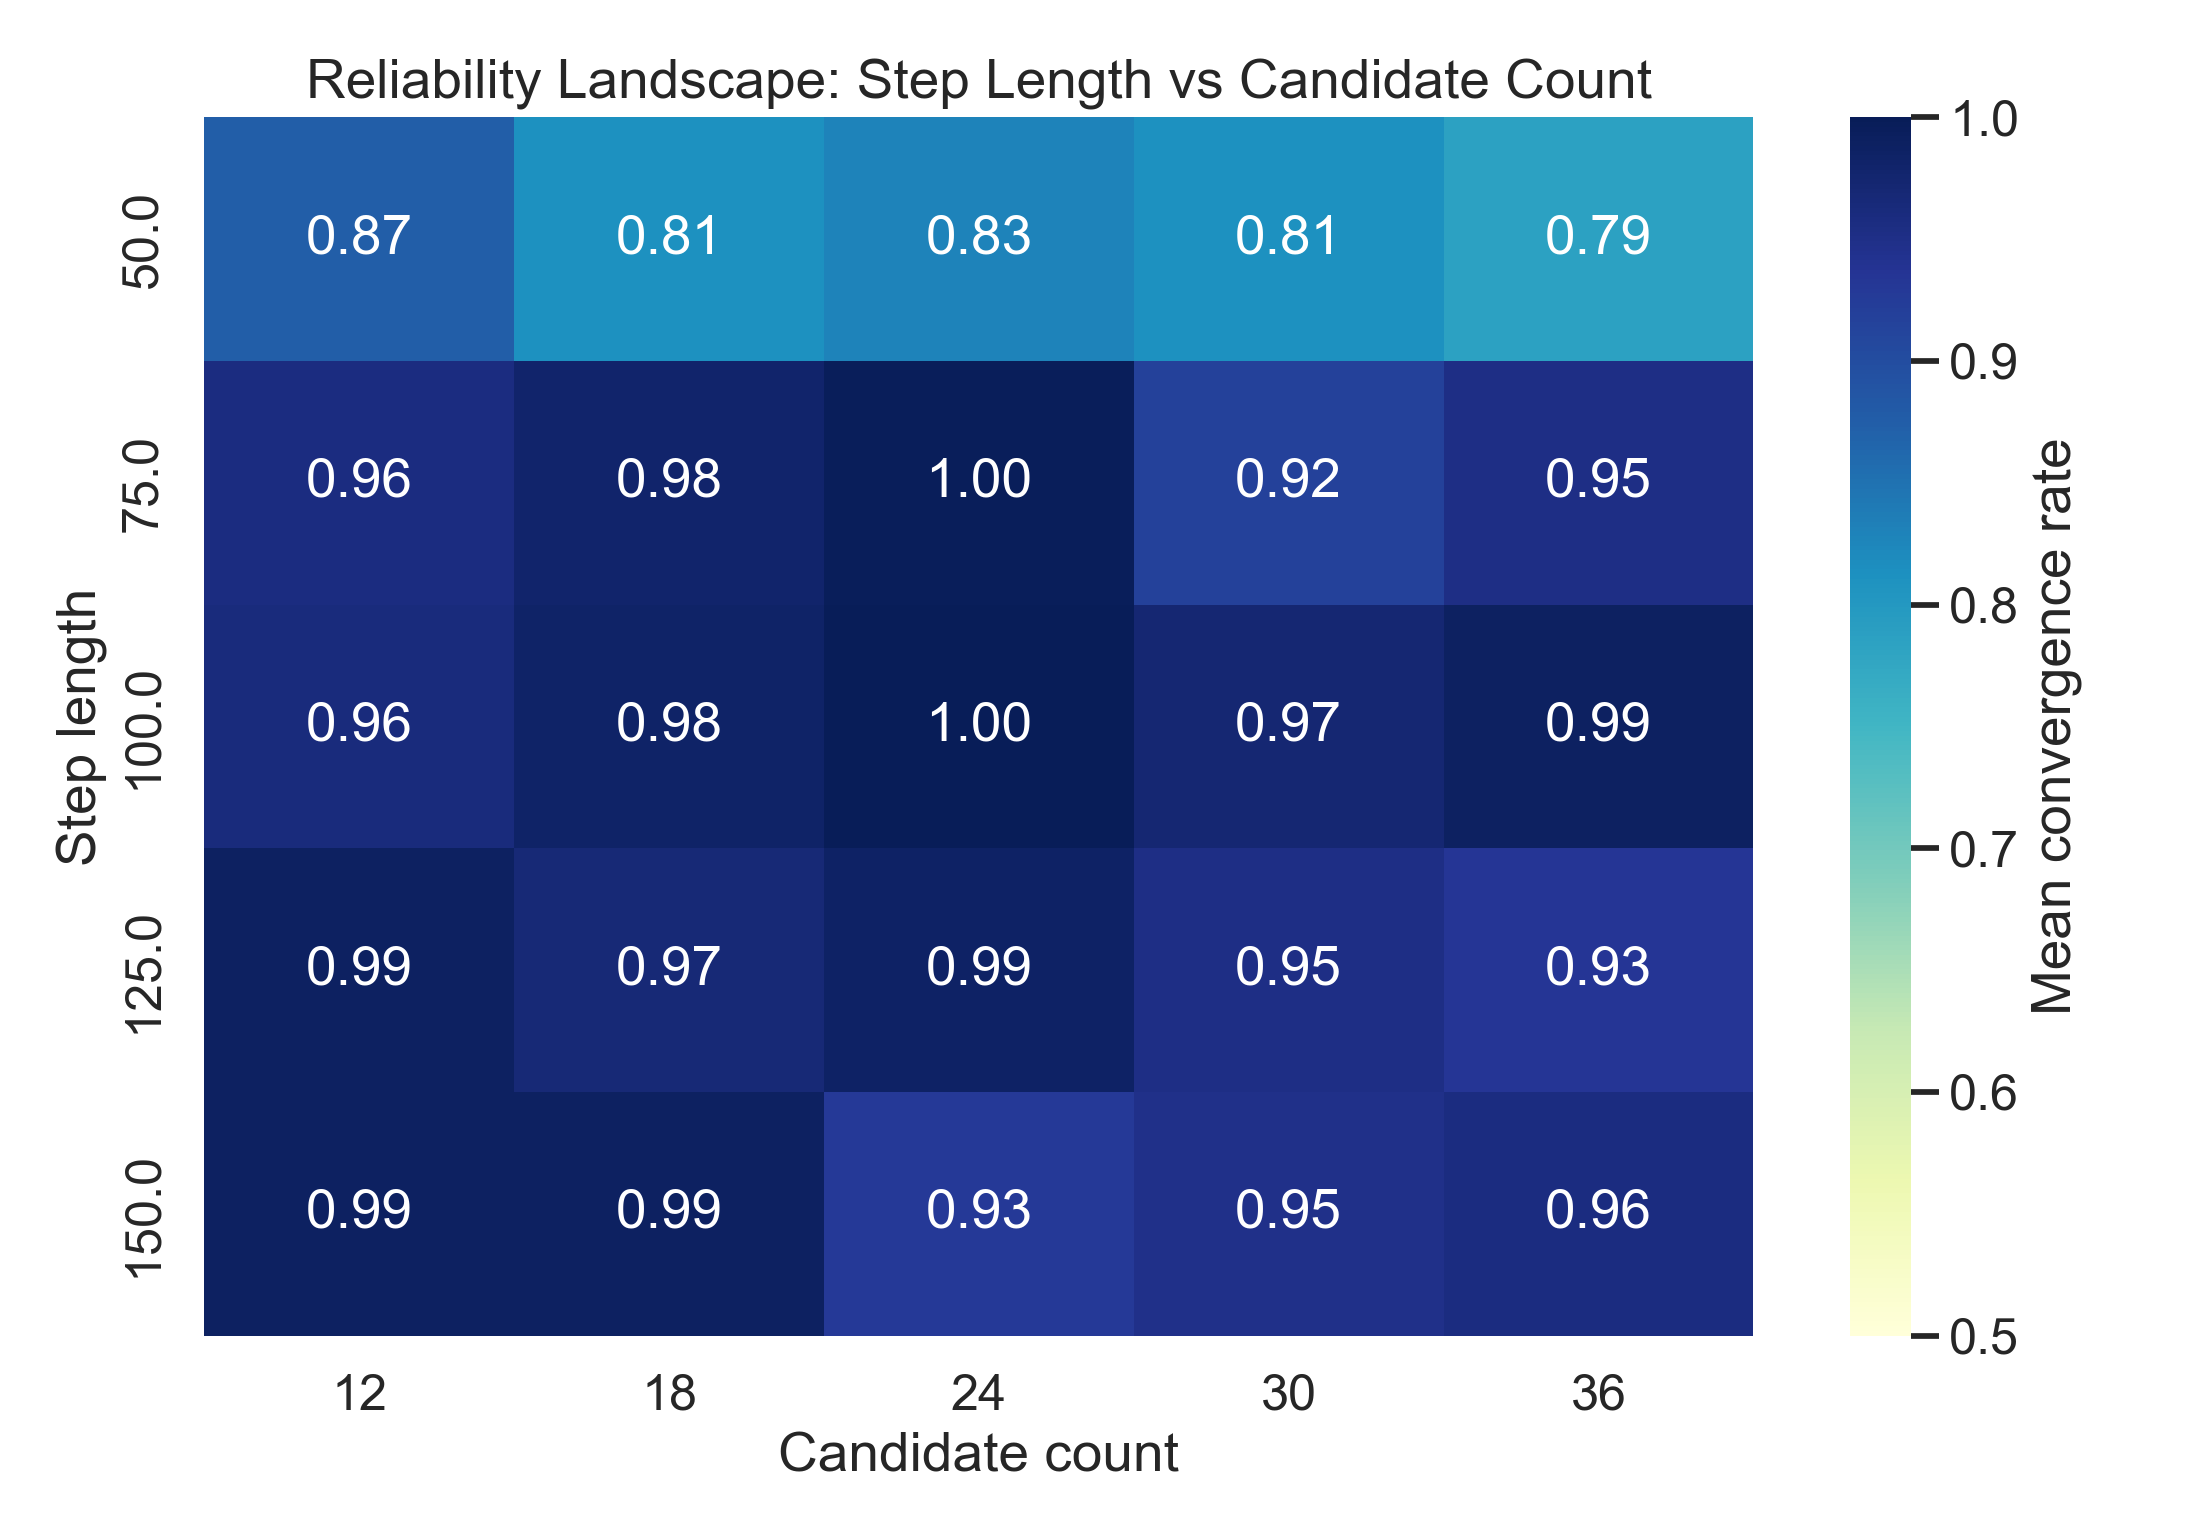
\includegraphics[width=0.49\textwidth]{img/experiments/full_factorial_20260601003651074/heatmap_step_candidate_rate.png}
    \hfill
    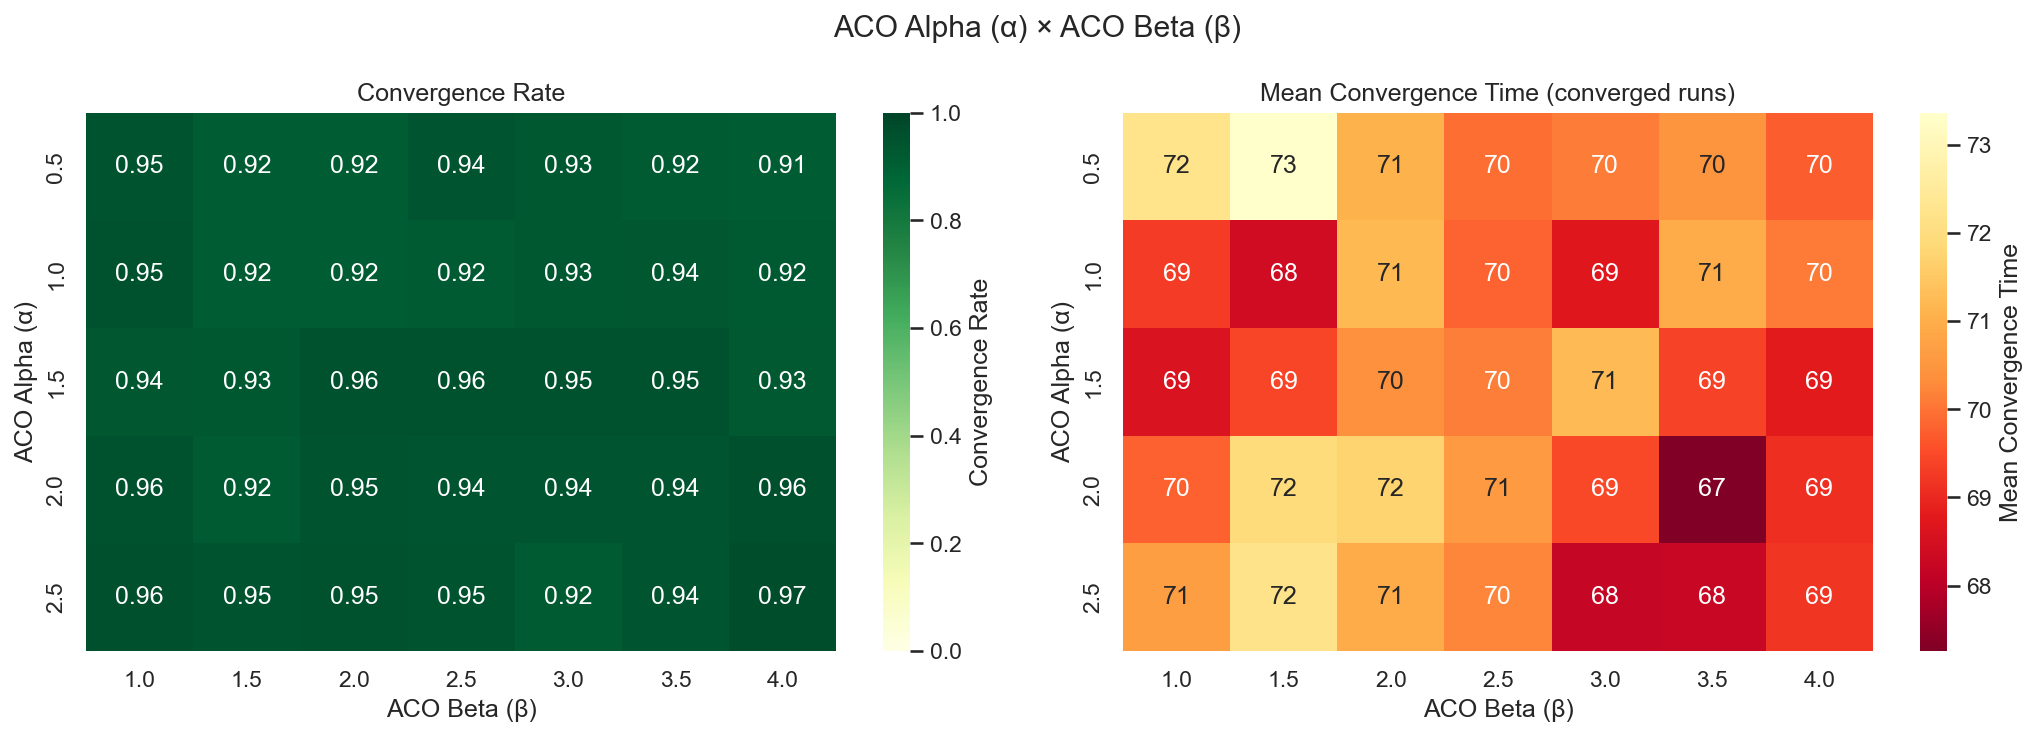
\includegraphics[width=0.49\textwidth]{img/experiments/full_factorial_20260601003651074/heatmap_alpha_beta.png}
    \caption{Full-factorial interaction views. Left: mean convergence rate over step length and candidate count. Right: reliability structure over $(\alpha,\beta)$. The dominant trough appears in short-step/high-candidate regions, while exponent effects are smoother and secondary.}
    \label{fig:fullfactorial_interactions}
\end{figure*}

\begin{figure*}[ht]
    \centering
    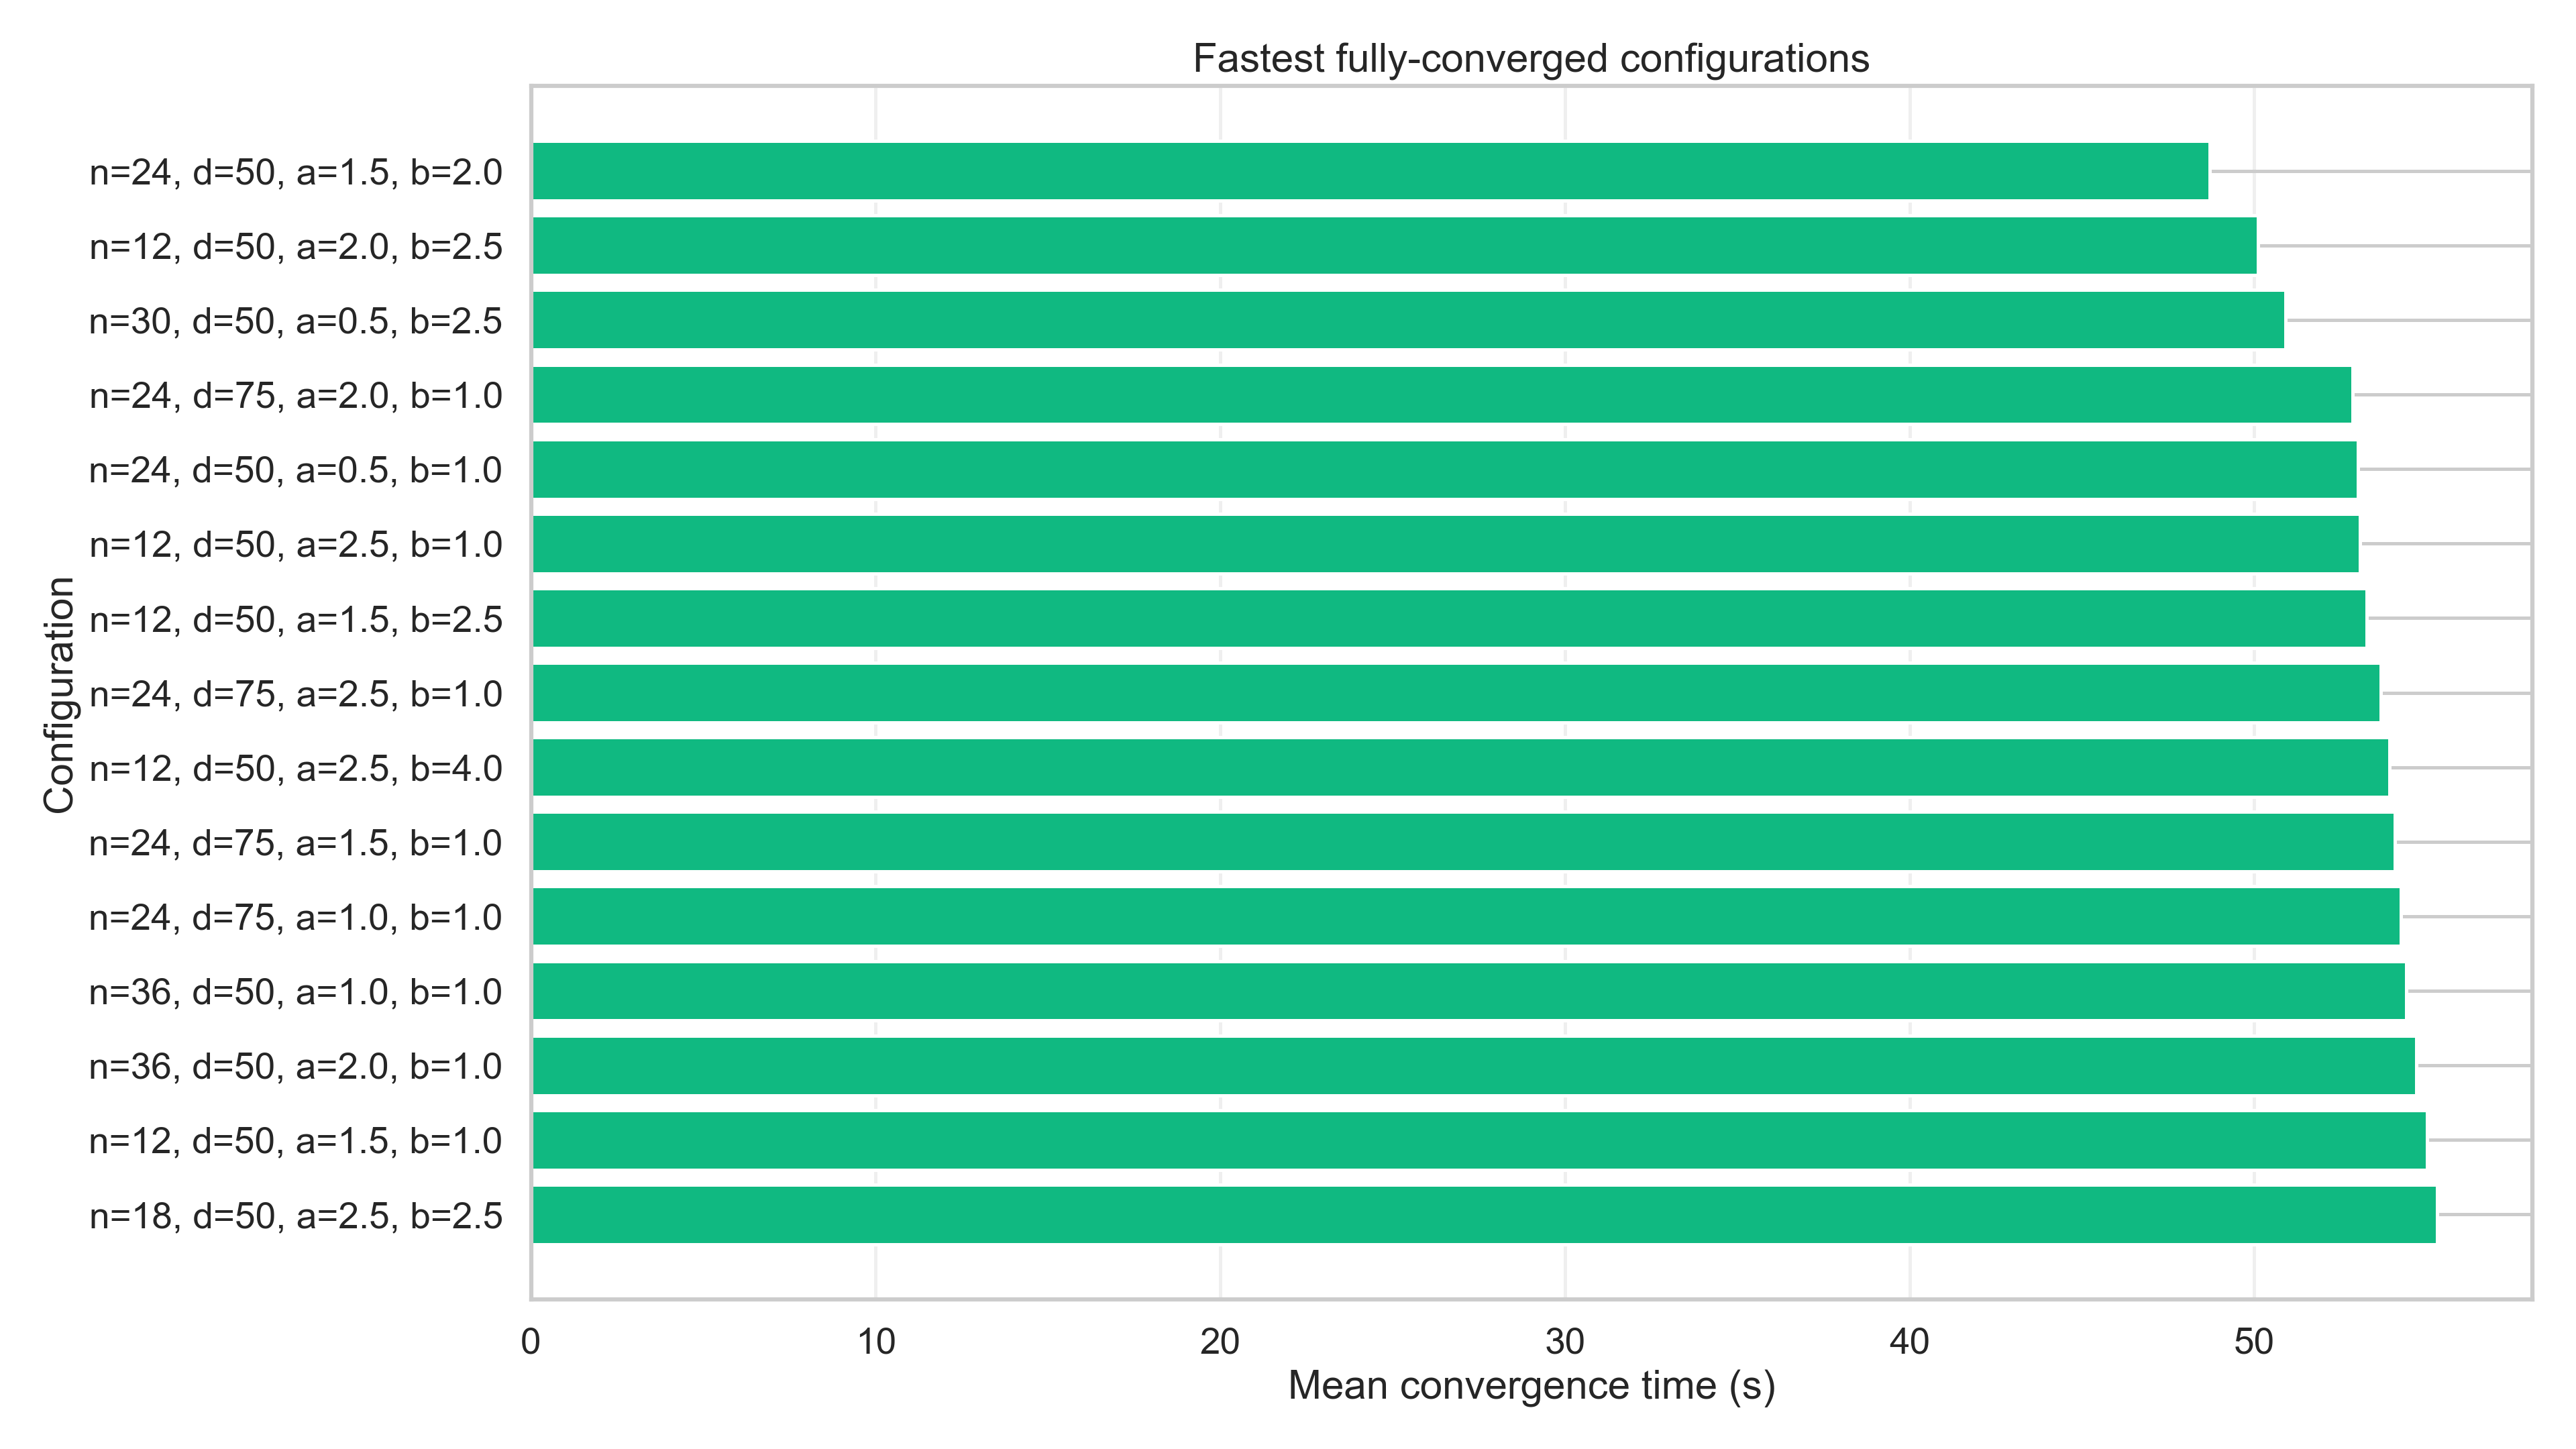
\includegraphics[width=0.49\textwidth]{img/experiments/full_factorial_20260601003651074/top15_full_converged.png}
    \hfill
    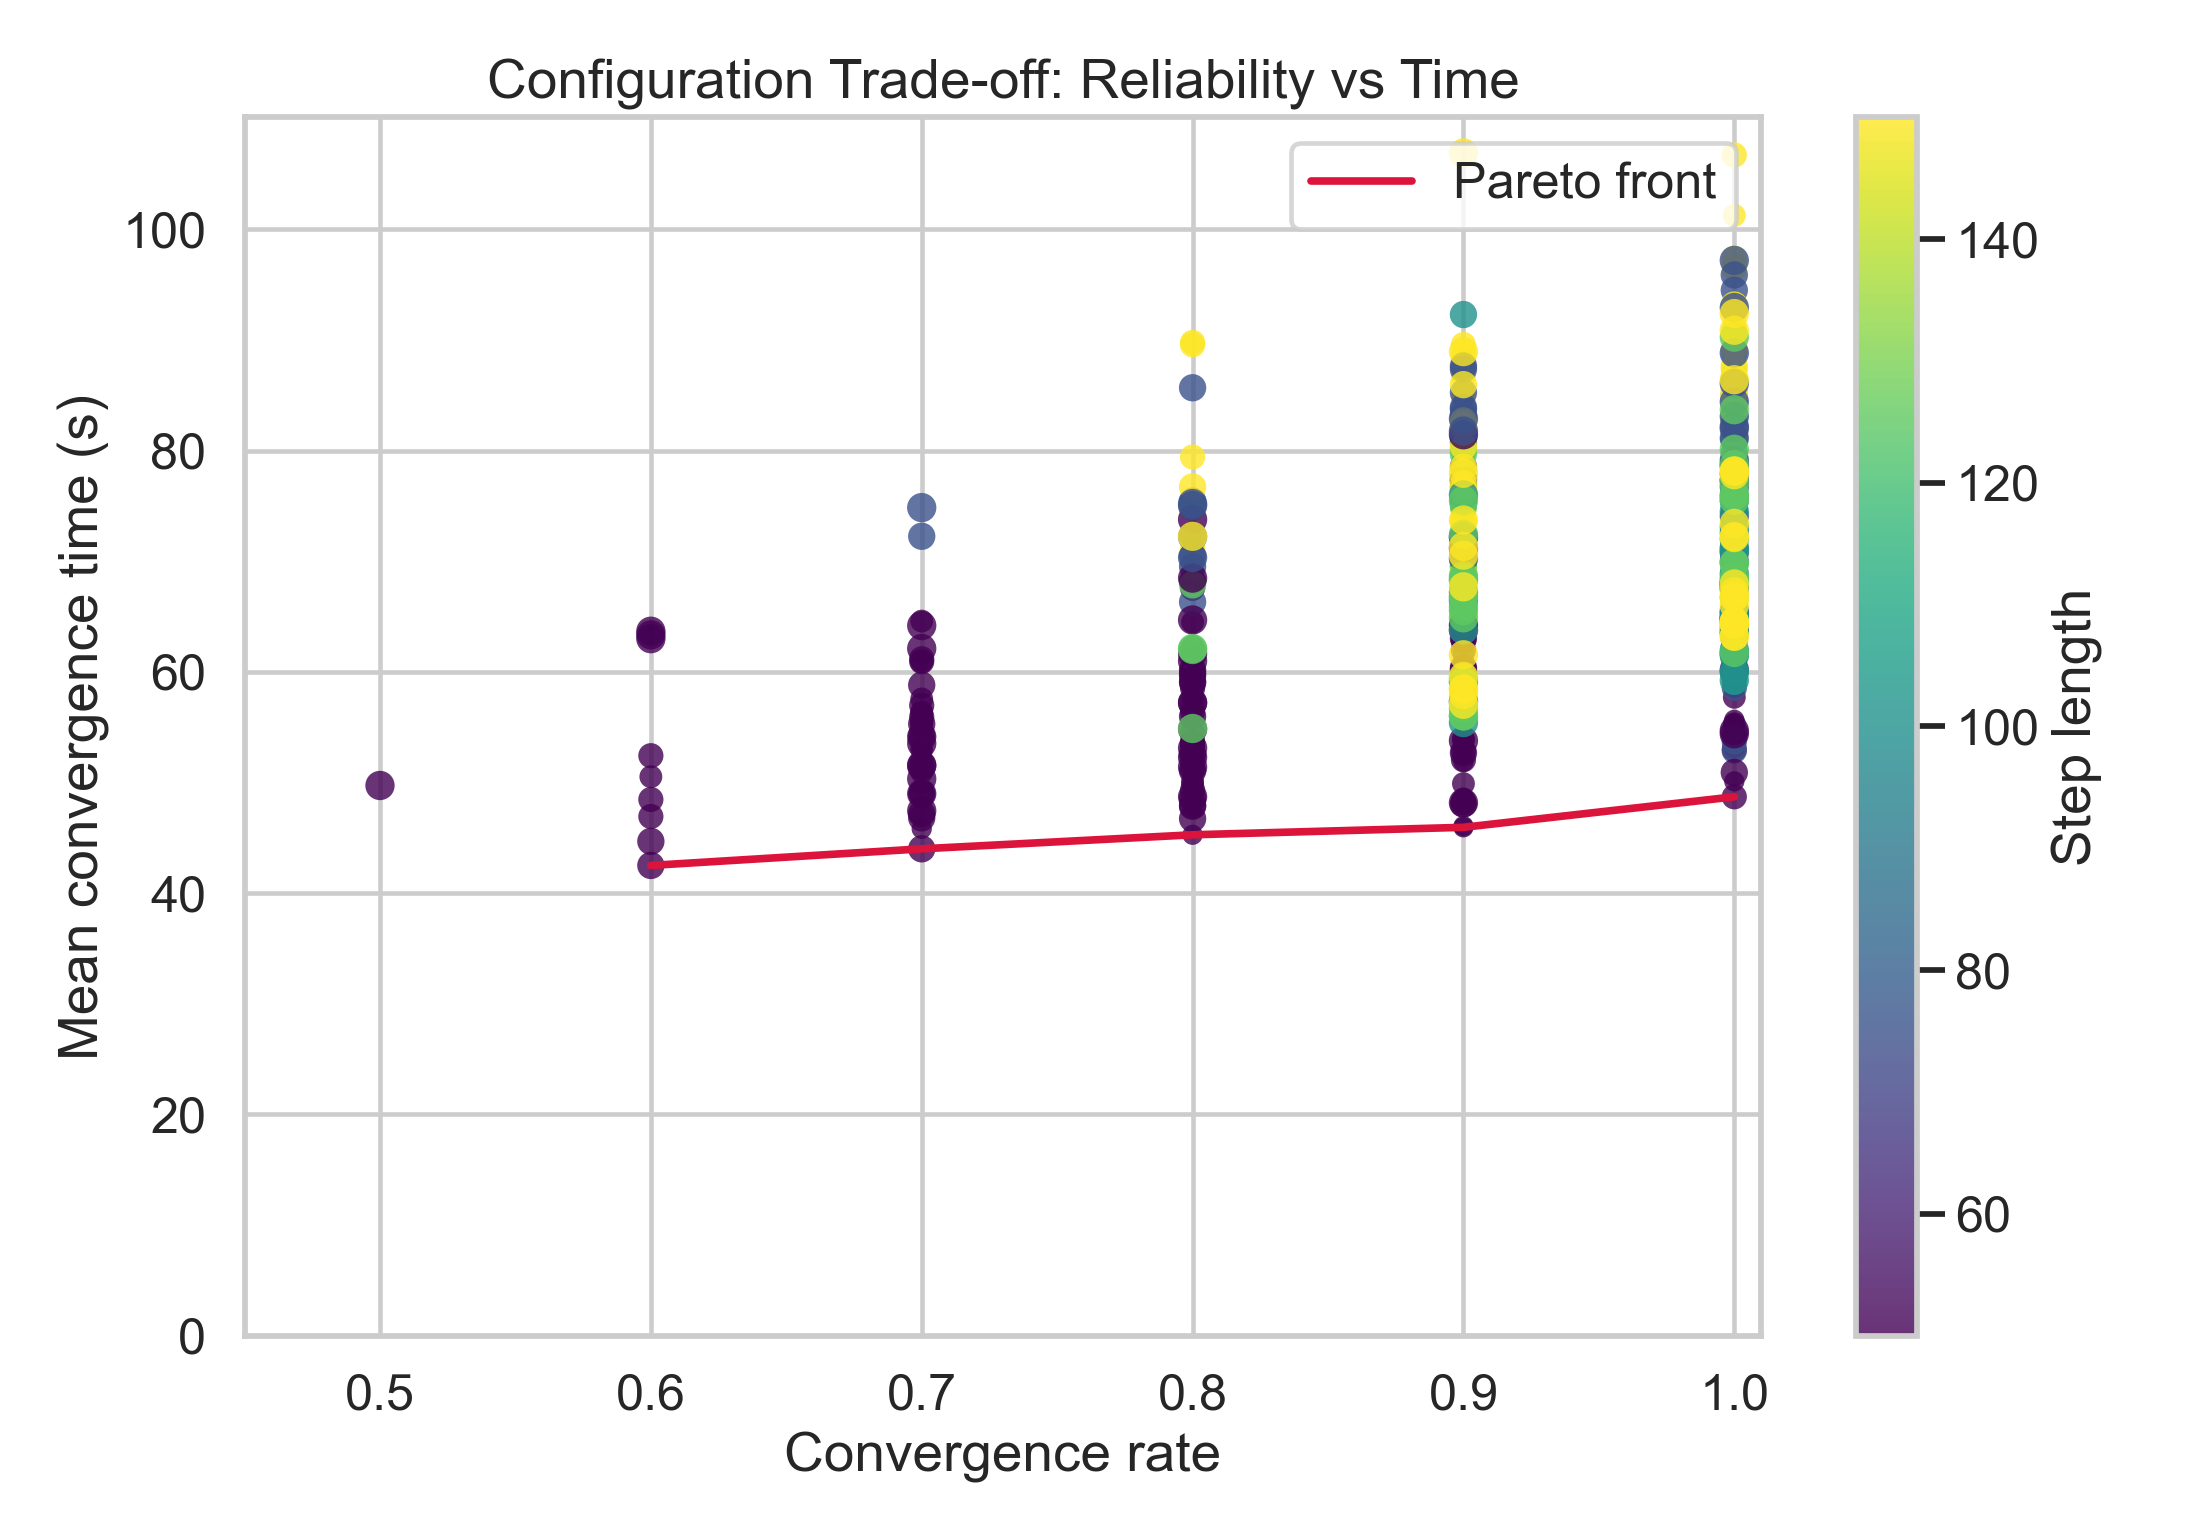
\includegraphics[width=0.49\textwidth]{img/experiments/full_factorial_20260601003651074/scatter_rate_vs_time.png}
    \caption{Summary diagnostics for the full-factorial sweep. Left: the fastest fully-converged configurations. Right: reliability--time trade-off across all 875 configurations with Pareto front overlay.}
    \label{fig:fullfactorial_tradeoff}
\end{figure*}

\subsection{Alpha--Beta Sensitivity}

A focused sweep over the ACO scoring exponents $(\alpha, \beta)$ in Equation~(2)
isolates how each term contributes to coverage performance. We vary both
exponents on the same grid $\{0.0, 0.5, 1.0, 1.5, 2.0, 2.5, 3.0\}$, deliberately
including the boundary at zero so the degenerate single-term scoring functions
appear as corner cases. This produces a $7 \times 7$ design of $49$ parameter
combinations. All other parameters are held at their defaults ($n = 24$,
$d = 4\,\text{m}$, sensor range $5\,\text{m}$), and each combination is
replicated over $21$ random seeds, giving $1029$ runs in total.

Convergence rate varies between $52\,\%$ and $76\,\%$ across the grid, and mean
convergence times among converged runs span $58$ to $71\,\text{s}$. The
dominant variation is along the $\beta$ axis. Columns with $\beta = 0$
consistently underperform, achieving only $52\text{--}57\,\%$ convergence;
once $\beta \geq 0.5$, convergence climbs into the $62\text{--}76\,\%$ band
and stays there. The $\alpha$ axis shows no comparable trend: at any fixed
$\beta \geq 1.0$, varying $\alpha$ from $0$ to $3$ shifts convergence rate by
at most $15$ percentage points and the response is non-monotonic. The worst
cell in the grid, $(\alpha, \beta) = (2.0, 0.0)$, achieves only $52\,\%$
convergence with a mean time of $70.6\,\text{s}$. The best convergence rates
($76\,\%$) appear at several cells, all with $\beta \geq 2.0$ and otherwise
unrelated $\alpha$ values, including $(0.0, 3.0)$, $(0.5, 2.0)$, and
$(2.5, 2.5)$. The fastest mean convergence times ($58\text{--}61\,\text{s}$)
cluster around moderate $\alpha$ and high $\beta$, with $(0.0, 3.0)$ and
$(0.0, 2.5)$ leading at roughly $61\,\text{s}$.

\begin{figure}[t]
  \centering
  
\includegraphics[width=0.95\columnwidth]{img/heatmap_alpha_beta.png}
  \caption{Convergence rate (left) and mean convergence time among
    converged runs (right) across the $7 \times 7$ grid of
    $(\alpha, \beta)$ values, $21$ seeds per cell. The $\beta = 0$
    column underperforms uniformly; $\alpha$ shows no comparable
    trend at fixed $\beta \geq 1$.}
  \label{fig:heatmap-ab}
\end{figure}

The asymmetry between $\alpha$ and $\beta$ follows directly from the scoring
function in our reversed-ACO formulation. Pheromone $\tau_i$ and freshness
$f_i$ are both updated inside the same \textsc{ExploreSense} tick: the same
sensor sweep that stamps a cell as freshly observed also deposits pheromone
on it. The two signals are therefore highly correlated, encoding the same
underlying fact (``this cell was visited recently'') in two different forms.
When $\beta > 0$, the staleness term $\eta_i^{\beta}$ already carries this
information, so further weighting the pheromone term through a larger $\alpha$
adds little independent directional signal. The $\beta = 0$ column is
qualitatively different because $\eta_i^{0} = 1$ collapses the staleness
contribution entirely, leaving the UAV with only the pheromone term, and
that signal alone is too coarse to consistently guide the swarm toward
unexplored ground.

This refines the broader observation made at the start of Section~6 that
$\beta$ has limited measurable effect. The effect is not absent: it has a
threshold structure. Moving from $\beta = 0$ to $\beta > 0$ measurably
improves convergence, but further increases past $\beta \approx 1$ provide
diminishing returns, consistent with our low-evaporation setup in which cells
never genuinely age out. No $(\alpha, \beta)$ cell achieved $100\,\%$
convergence across all $21$ seeds, indicating that the seed-to-seed variance
in GMM victim placement imposes a ceiling that local rule choices alone
cannot lift. For practical use, the default $(\alpha, \beta) = (1.0, 2.0)$
sits inside the high-convergence region of the grid, and the model is
largely insensitive to small departures from it.
